\documentclass{article}
\usepackage[magyar]{babel}
\usepackage{t1enc}
\usepackage{lipsum}
\usepackage{hulipsum}
\usepackage{tikz}
\usetikzlibrary{patterns}


\begin{document}

\tikz{ \fill[red] (0,0) circle (1);
\filldraw[draw=green,fill=yellow,opacity=0.8,
fill opacity=0.3] (1,0) circle (1); }

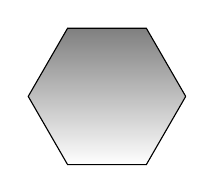
\begin{tikzpicture}

   \newdimen\R
\R=1cm
   \filldraw[draw=black, fill=black, shading=axis] (0:\R)
   \foreach \x in {60,120,...,360} {  -- (\x:\R) }
 ;
\end{tikzpicture}

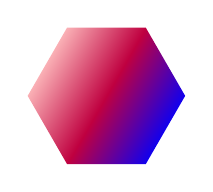
\begin{tikzpicture}
\newdimen\R
\R=1cm
\shade[top color=pink, bottom color=blue,
middle color=purple, shading angle=60]
(0:\R)
   \foreach \x in {60,120,...,360} {  -- (\x:\R) };
\end{tikzpicture}


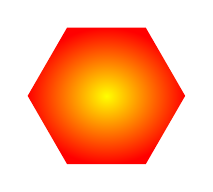
\begin{tikzpicture}
\newdimen\R
\R=1cm
\shade[shading=radial, outer color=red,
inner color=yellow]
(0:\R)
   \foreach \x in {60,120,...,360} {  -- (\x:\R) };
\end{tikzpicture}


\begin{tikzpicture}
\newdimen\R
\R=1cm
\newcommand{\utvonalam}{(0,0) -- ++(45:1) -- ++(135:1) -- ++(225:1) -- (0,0);}
\fill[blue] \utvonalam ;
\pattern[pattern=fivepointed stars,
pattern color=white] \utvonalam ;
\end{tikzpicture}

\tikz{\shade[shading=ball, ball color=red]
(0,0) circle (0.5);}


\end{document}